\documentclass[12pt,a4paper]{article}
\usepackage{graphicx}
\usepackage{amsmath}
\usepackage{amssymb}
\usepackage{subfigure}
\usepackage{booktabs}
\usepackage{color}
\usepackage{listings}
\usepackage{eurosym}
\usepackage{mathtools} % for \mydef
\usepackage{float}
\usepackage{natbib}
\usepackage{gensymb} % for \degree
%\usepackage{authblk} % for multiple authors with different affiliations
\usepackage[small]{titlesec}
\usepackage[displaymath, mathlines]{lineno}

% see http://tex.stackexchange.com/questions/99316/symbol-for-external-links
\usepackage{fontawesome}
\usepackage[hidelinks]{hyperref}
% Redefinition, symbol included in link:
\let\orighref\href
\renewcommand{\href}[2]{\underline{\orighref{#1}{#2}}}
% hyphens option for hyperref: enables line-breaks at hyphens. Otherwise only at slashes /. Ugly
%\PassOptionsToPackage{hyphens}{url}\usepackage{hyperref}

\addtolength{\oddsidemargin}{-2cm}
\addtolength{\evensidemargin}{-2cm}
\addtolength{\textwidth}{4cm}
\addtolength{\topmargin}{-2cm}
\addtolength{\textheight}{2cm}

%%%%%%%%%%%%%%%%%%%%%%%%%%%%%%%%%%%%%%%%%%%%%%%%
% REMOVE FOR FINAL VERSION


%%DRAFT HEADERS on normal pages
%\usepackage{fancyhdr}
%\pagestyle{fancy}
%\fancyhf{} % clear all headers and footers
%\fancyhead[C]{{\bf DRAFT}}
%\cfoot{\thepage}
%%DRAFT HEADERS on TOC and Chapter pages
%\fancypagestyle{plain}{
%	\fancyhf{}
%	\fancyhead[C]{{\bf DRAFT}}
%	\cfoot{\thepage}
%}
%%DRAFT HEADERS on title pages
%\fancypagestyle{empty}{
%	\fancyhf{}
%	\fancyhead[C]{{\bf DRAFT}}
%}

%%%%%%%%%%%%%%%%%%%%%%%%%%%%%%%%%%%%%%%%%%%%%%%%%%%%%%%%


\renewcommand{\familydefault}{\sfdefault}

\graphicspath{{../figures/}} 

%\linenumbers

\title{
	{\bf DRAFT}\\
	Notes on running ROMS on Amazon Web Services 
}

\author{Stefan Riha\thanks{Email: stefan@sriha.net}}
%\date{}

\begin{document}
	\setlength{\parindent}{0cm}
	\maketitle
	
\section{Introduction}

The Regional Ocean Modeling System \citep[ROMS, see ][]{shchepetkin2005regional} provides three benchmark tests, consisting of 
an idealized model of the Southern Ocean with three grid sizes:

\begin{itemize}
	\item \verb|benchmark1|:   512 x 64 x 30 grid points
	\item \verb|benchmark2|:   1024 x 128 x 30 grid points
	\item \verb|benchmark3|:   2048 x 256 x 30 grid points
\end{itemize}

All experiments are integrated for 200 time steps. No grid data is read or written from/to the hard disk.

\section{Preliminary results}
	All results shown were produced with ROMS compiled with Open MPI using gfortran.
	
	\begin{figure}[H]
		\centering
		\includegraphics[width=0.5\textwidth]{met_t2micro.pdf}
		\caption{Time (in seconds) spent per process for the ROMS "small" benchmark test (benchmark1.in), as function of the number of processes. Axes are logarithmic with base 2. Computations are performed on t2.micro instances of AWS, which have one vCPU per (virtual) node (2016/11/01). Each data point shows the average over all processes, measured from one single experiment. The inset shows the domain partition (tiling) of the 512x64(x30) point domain. The result suggests that partitioning along the first dimension yields better performance.}
		\label{fig:met_t2micro}
	\end{figure}

	\begin{figure}[H]
	\centering
	\includegraphics[width=0.5\textwidth]{met_c4large.pdf}
	\caption{Same as Fig. \ref{fig:met_t2micro}, but computations are performed on c4.large instances of AWS, which have 2 vCPUs per (virtual) node. In the case of c4 instances, a vCPU is defined as a single thread of a custom 2.9 GHz Intel Xeon E5-2666 v3 (Haswell) processor (2016/11/01).}
	\label{fig:met_c4large}
\end{figure}

\begin{figure}[H]
	\centering
	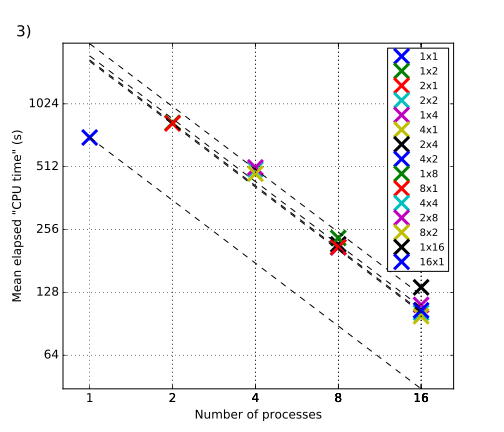
\includegraphics[width=0.5\textwidth]{met_c44xlarge.pdf}
	\caption{Time (in seconds) spent per process for the ROMS "medium" benchmark test (benchmark2.in), as function of the number of processes. Computations are performed on c4.4xlarge instances of AWS, which have 16 vCPUs per (virtual) node.}
	\label{fig:met_c44xlarge}
\end{figure}

\begin{figure}[H]
	\centering
	\includegraphics[width=0.5\textwidth]{met_c48xlarge.pdf}
	\caption{Time (in seconds) spent per process for the ROMS "large" benchmark test (benchmark3.in), as function of the number of processes. Computations are performed on c4.8xlarge instances of AWS, which have 32 vCPUs per node.}
	\label{fig:met_c48xlarge}
\end{figure}

\subsection{Computational and monetary costs of a realistic study}

The preliminary test above allow a rough estimate of the computational and monetary costs involved in a realistic study. By monetary cost we mean the financial cost of renting AWS' hardware to conduct a study of a given computational cost. As an example we consider \cite{kumar2015midshelf}, who validate the midshelf and surfzone circulation generated by a numerical model against observations.  They use a coupled ROMS-SWAN model and compare it to observations from the 2006 Huntington Beach (San Pedro Bay, California, U.S.A.) experiment. We assume that such studies, which investigate the transport processes directly adjacent to the coast, are particularly important for commercial applications. Whether or not it is actually \emph{technically feasible} to conduct such a highly complex state-of-the-art simulation on AWS' cloud infrastructure, is not shown here. Instead, the objective here is to gain a (very rough) order-of-magnitude estimate of the involved cost, \emph{assuming} technical feasibility. 

\subsubsection{Components of the numerical experiment}

The numerical experiment of \cite{kumar2015midshelf} consists of the following components:

\begin{itemize}
	\item Wind forcing
	\item Wave forcing
	\item Tide forcing
	\item Buoyancy forcing
\end{itemize}

which are coupled by the open-source Coupled Ocean-Atmosphere-Wave-Sediment (COAWST) Transport model \citep{warner2008using,web:coawst}, which couples an atmospheric (Weather Research and Forecasting model, WRF), wave (SWAN), three-dimensional circulation and stratification (ROMS) and sediment transport models. COAWST is integrated by the Model Coupling Toolkit (MCT, \citealt{web:mct}) to exchange data fields between the models. They use the following nested grids:

\begin{itemize}
	\item U.S. West Coast and eastern Pacific (L0):  $\Delta=5\,\rm km$, area $4000\times3000\,\rm km^2$ ($800\times600\times40$ grid points)
	\item Southern California Bight (L1):  $\Delta=1\,\rm km$, area $800\times700\,\rm km^2$ ($800\times700\times40$ grid points)
	\item Interior bight region (L2): $\Delta=250\,\rm m$, area $500\times300\,\rm km^2$ ($2000\times1200\times40$ grid points)
	\item San Pedro Bay (L3): $\Delta=75\,\rm m$, area $80\times70\,\rm km^2$ ($1067\times934\times32$ grid points)
	\item Huntington Beach, Newport Beach (shelf break to inner shelf and surfzone): $\Delta=50\,\rm m$, area $15\times30\,\rm km^2$ ($214\times428\times20$ grid points)
	\item Huntington Beach (mid-shelf to surfzone): $\Delta=10\,\rm m$, area $6\times6\,\rm km^2$ ($600\times600\times20$ grid points)
\end{itemize}

 As boundary conditions (forcing fields) they use\footnote{\cite{kumar2015midshelf} provide an overview of their model set up, but understandably don't provide full detail. Our presentation may be inaccurate.}

\begin{itemize}
	\item Lateral forcing: The parent grid L0 is forced with a combination of lateral boundary conditions from an assimilated global oceanic dataset \citep{carton2008reanalysis}. Freshwater flux from river runoff is included. In addition, barotropic tidal elevation and velocities are projected onto the boundaries of L1.
	
	\item Surface forcing (wind-stress, heat, radiative and freshwater) is provided by a doubly nested WRF model with $\Delta=18\,\rm km$ (for L0) and $\Delta=6\,\rm km$ (for L1, L2, L3), embedded within the NCEP North American Regional Reanalysis. Surface temperature and salinity are relaxed to monthly averages from \cite{carton2008reanalysis}.
	
\end{itemize}

The L0-L5 domains are one-way nested, i.e. L0-L4 each provide boundary condition data for their respective child grid. Daily L0 solutions are used as a lateral boundary condition for L1. L1 (L2) solutions are used as L2 (L3) lateral boundary conditions every $2\,\rm h$. Note again that L1's boundary condition includes barotropic tidal elevation and velocities in addition to information provided by its parent.

The model is spun up for $15\,\rm yr$ with climatological surface forcing.


For time-stepping the shelf grids, \cite{kumar2015midshelf} state that

\begin{itemize}
	\item L4 and L5 are integrated for 92 days with a baroclininc time step of $8\,\rm s$ and $4\,\rm s$, respectively.
	\item wave action density in SWAN evolves with a time step of $120\,\rm s$ and $60\,\rm s$, respectively. Exchange of information between the circulation and wave models occurres every $360\,\rm s$.
\end{itemize}


\subsubsection{Computational cost}

\cite{kumar2015midshelf} do not report the time step used in their L0-L3 models. Assuming an ocean depth of $H=2000\,\rm m$, the barotropic time step is constrained by the CFL condition to roughly $\mathcal{O}(10\,\rm s)$ for L0 and L1, and $\mathcal{O}(1\,\rm s)$ for L2 and L3, according to the simplified formula (which does not hold strictly in this practical application)

\begin{equation}
\Delta t_{b}\leq\Delta x/c \qquad c=\sqrt{gH},
\end{equation}

where $\Delta t_b$ ($\Delta x$) is the barotropic time step (lateral grid spacing), and $g$ is standard gravity. Assuming that the baroclinic time step $\Delta t$ is a factor of 10-20 longer than the barotropic time step, this yields $\Delta t=\mathcal{O}(100\,\rm s)$ (L0, L1) and $\Delta t= \mathcal{O}(10\,\rm s)$ (L2, L3), respectively. For a $15\,\rm yr$ simulation, $N=\mathcal{O}(10^7)$ baroclinic time steps are required. Clearly, these estimates are very rough. For example, to account for the shallower depth of the L2 and L3 grids,  one may assume a depth decrease by a factor of 10, and accordingly increase $\Delta t_b$ by a factor of 3 for L2 and L3. 

So far, no results are available measuring execution time for grids of similar size as L0-L3. The closest matching available result is for \verb|benchmark2|, with a grid size of $1024$x$128$x$30$ data points, which is roughly 1/10 of the number of spatial data points in L0-L3. Note that it is always possible to assume identical physical dimensions of the grid spacing (including the temporal lattice) between \verb|benchmark2| and L0-L3, since the benchmarking results are independent on physical dimensions (but depend only on the amount of data points).


\subsubsection{Monetary cost}

Hence, in the following we may assume $\Delta t$ and $\Delta x$ is similar for \verb|benchmark2| and L0-L3, keeping in mind that the amount of processed data is an order of magnitude less than for each of the 4 experiments L0-L3.
Fig. \ref{fig:met_c44xlarge} shows that \verb|benchmark2| takes roughly $100\,\rm s$ to complete on a 16-core \verb|c4_4xlarge| instance using the gfortran compiler. The number of time steps integrated in  \verb|benchmark2| is 200, i.e. about 2 time steps per second are processed. It follows that a $15\,\rm yr$ spin up time for \verb|benchmark2| takes roughly $\mathcal{O}(60\,\rm d)$ to complete.

The instance type \verb|c4_4xlarge| is currently (2017/01/12) priced at \textdollar 0.796 per hour for on-demand use, resulting in a total of $\mathcal{O}($\textdollar $1,000) $ for a 2 month lease.


\subsection{TODO}

\begin{itemize}
	\item Relate monetary cost of computations to cost of labor?
\end{itemize}

	
\bibliography{main.bib}
\bibliographystyle{model2-names}

\end{document}

 
